%!TEX root = ../dokumentation.tex

\chapter{Versuchsumgebung}
\todo[inline]{Einführung in Kapitel Versuchsumgebung}

\section{Aufbau}
Um die Verwendung von Eye-Tracking zur Steuerung von Bedienelementen in \ac{VR} untersuchen zu können, finden die Versuche in einem leeren neutralen Raum statt. Dies hat den Vorteil, dass der Benutzer von der kompletten \ac{VR}-Welt abgeschirmt ist. Der Benutzer kann sich daher besser auf den Versuch fokussieren, da dieser nicht durch eventuell neu gewonne Eindrücke aus der \ac{VR}-Welt abgelenkt wird. Um Ablenkungen bezüglich Farbwechsel an den Wänden, dem Boden oder der Decke zu vermeiden, erhalten diese Elemente die gleiche Hintergrundfarbe. Zudem wird der Raum gleichmäßig beleuchtet. Für eine bessere Vergleichbarkeit der Versuchsergebnissen muss der Benutzer bei jedem Versuch auf der gleichen Position im Raum stehen. Diese Position wird auf dem Boden durch ein rotes Quadrat markiert (siehe \autoref{fig:game-plan}). Vor Beginn des Versuches muss sich der Benutzer auf dem roten Quadrat positionieren. Dies wird benötigt, da der Benutzer die Möglichkeit hat, sich innerhalb einer vom \ac{VR}-Headset berechneten Spielfläche zu bewegen. Dieses Quadrat befindet sich mittig zentriert circa eine halbe Einheit vor einer Wand. Das Quadrat hat eine Seitenlänge von einer halben Einheit.

Zur Untersuchung der Eignung von Eye-Tracking bei der Steuerung von Bedienelementen befindet sich auf der gegenüberliegenden Wand die Versuchsfläche (siehe \autoref{fig:game-view}). Der Versuch ist wie ein Spiel aufgebaut. Der Benutzer muss fünf zufällige Zahlen von 1 bis 16 nacheinander auswählen. Auf der Spielfläche befinden sich 16 Bedienelemente, die mit Zahlen von 1 bis 16 beschriftet sind. Oberhalb der Bedienelemente befindet sich ein Textfeld, welches dem Benutzer die auszuwählende Zahl mitteilt. Zudem teilt das Textfeld das Ende des Spieles mit. Um das Spiel zu starten, muss der Benutzer den GO-Button betätigen. Beim Betätigen eines Bedienelementes wird die Hintergrundfarbe des Elements verändert. Dies wird in Abhängigkeit der gesuchten Zahl und des ausgewählten Elements festgelegt. Wenn die gesuchte Zahl und die Beschriftung des ausgewählten Bedienelements übereinstimmen, wird das Element grün gefärbt, ansonsten rot.

\begin{figure}[!htbp]
	\centering
	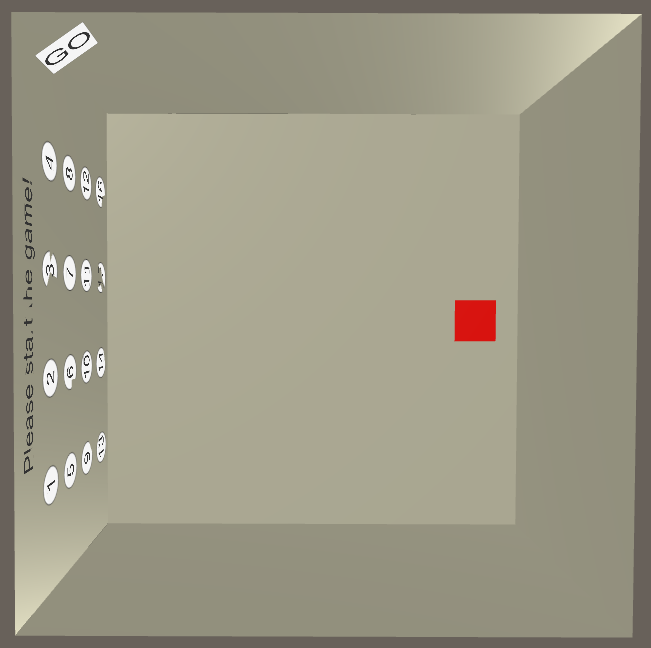
\includegraphics[width=0.65\linewidth]{game-plan}
	\caption[Draufsicht auf den Raum]{Draufsicht auf den Raum}
	\label{fig:game-plan}
\end{figure}

\begin{figure}[!htbp]
\centering
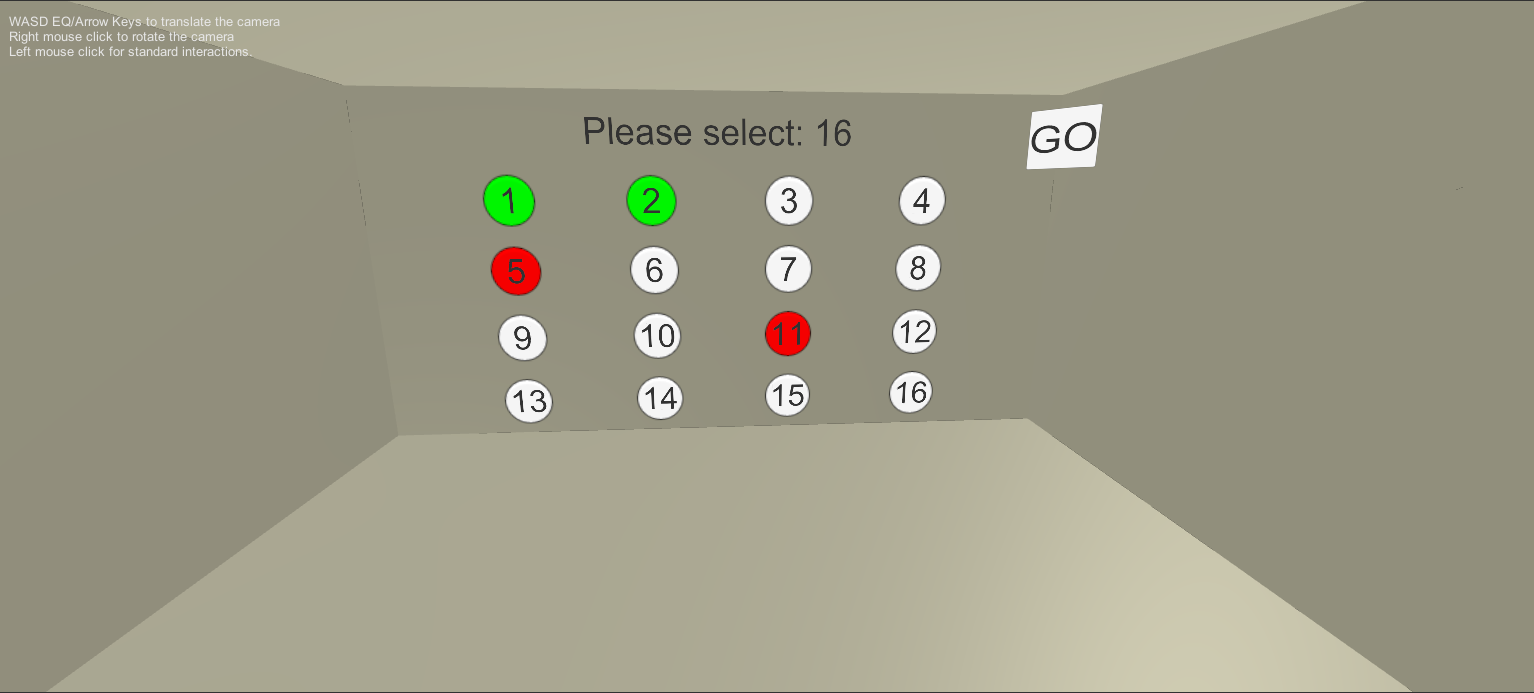
\includegraphics[width=1\linewidth]{game-view}
\caption[Benutzersicht auf den Versuch]{Benutzersicht auf den Versuch}
\label{fig:game-view}
\end{figure}

\section{Szenen}
\todo[inline]{Sinnvoll von Metern zu reden oder doch lieber von Einheiten?}
\todo[inline]{Erklären wieso die Szenen so aufgebaut wurden? Z.B. warum verschiedene Entfernungen? Und wieso das 3D-Level?}
\todo[inline]{Bezug auf Forschungsfrage}
Für die Versuche existieren vier verschiedene Szenen. Jede Szene basiert auf dem zuvor beschriebenen Aufbau. Jeder der Räume ist 2,5 Meter hoch und 5 Meter breit. In der ersten Szene \glqq FittsLaw\grqq (siehe \autoref{fig:game-view}) steht der Benutzer 4,5 Meter von der gegenüberliegenden Wand entfernt. In der zweiten Szene \glqq FittsLawFar\grqq (siehe \autoref{fig:FittsLawFar}) und der dritten Szene \glqq FittsLawFurther\grqq (siehe \autoref{fig:FittsLawFurther}) wurde die Entfernung zwischen Benutzer und Spielfläche jeweils um 2,5 Meter zur vorherigen Szene vergrößert. Die vierte und letzte Szene \glqq 3D-Level\grqq (siehe \todo{Verweis auf Abbildung}) basiert auf der Szene FittsLawFurther. Der Unterschied ist jedoch, dass sich die Buttons nicht mehr an der Wand befinden sondern frei im Raum schweben. 

\begin{figure}[!htbp]
	\centering
	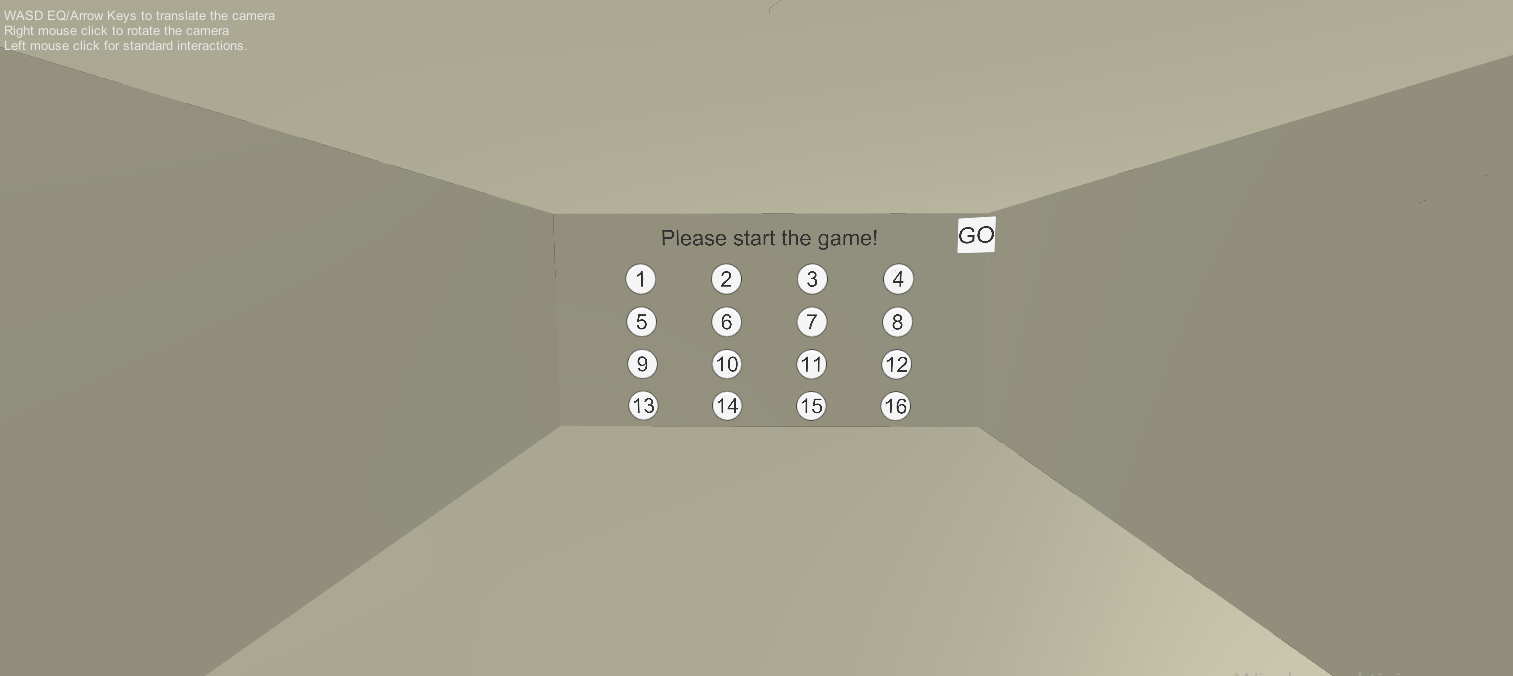
\includegraphics[width=1\linewidth]{FittsLawFar}
	\caption[Szene FittsLawFar]{Szene FittsLawFar}
	\label{fig:FittsLawFar}
\end{figure}

\begin{figure}[!htbp]
	\centering
	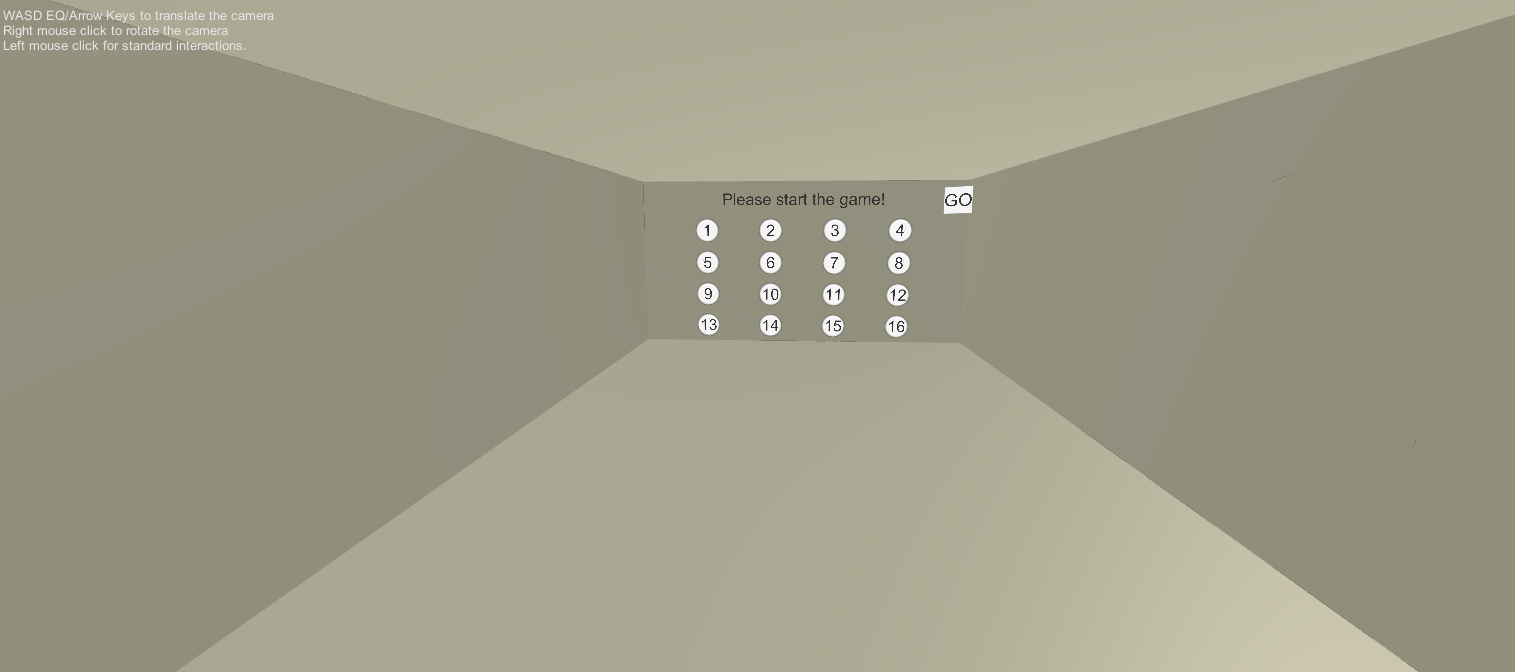
\includegraphics[width=1\linewidth]{FittsLawFurther}
	\caption[Szene FittsLawFurther]{Szene FittsLawFurther}
	\label{fig:FittsLawFurther}
\end{figure}

\missingfigure{Szene 3D-Level: Muss Clemens machen. Ich kann leider den Button nicht aktivieren}

\section{Implementierung}
\missingfigure{Klassendiagramm}
wichtigste Klassen erklären \\

4 Wände: komplett Beleuchtet; nur nach vorne Beleuchtet \\

Measurement \\
Auswahl: Laser oder Trigger; EyeTrigger / Blink Detection; Größe Verstellbar \\

\begin{figure}[!htbp]
	\centering
	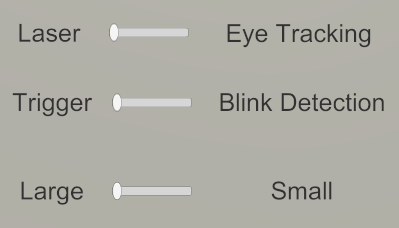
\includegraphics[width=1\linewidth]{switch-different-options}
	\caption[Einstellungsoberfläche für die Versuchsoptionen]{Einstellungsoberfläche für die Versuchsoptionen; Oben: Auswahl; Mitte: Trigger; Unten: Größe der Buttons}
	\label{fig:switch-different-options}
\end{figure}